\chapter{Stabilization}
%
%\begin{figure}[H]
%  \hspace{-10pt}
%  \captionbox 
%  {
%    a
%    \label{fig:Edelta_twinSwingAndCatch}
%  }
%  {
%    \hspace{-1cm}
%    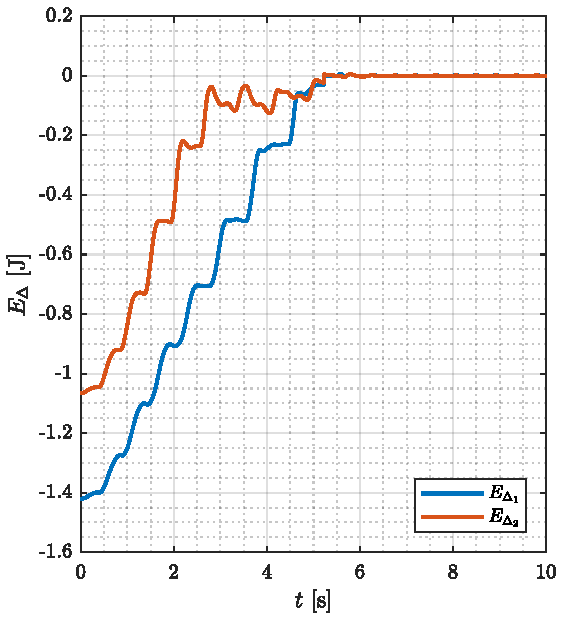
\includegraphics[width=.448\textwidth]{figures/Edelta_twinSwingAndCatch}
%  }
%  \hspace{20pt}
%  \captionbox 
%  {
%    a
%    \label{fig:phase_twinSwingAndCatch}
%  }
%  {
%    \hspace{-1cm}
%    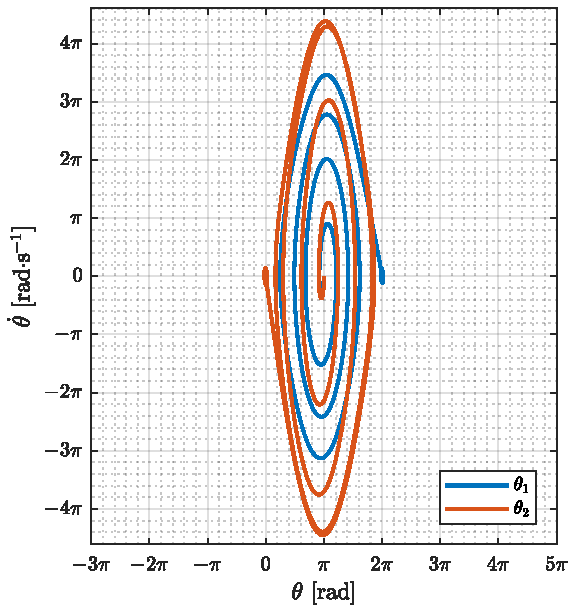
\includegraphics[width=.46\textwidth]{figures/phase_twinSwingAndCatch}
%  }
%\end{figure}
%
In this chapter a Linear Quadratic Regulator (LQR) is designed to stabilize the twin pendulum in upright position taking over from the swing-up controller.\\
The nonlinear state space system from \autoref{eq:nonlinearStateSpaceTwin} are linearized,
\begin{align}
  A &= \frac{\partial \vec{f(x)}}{\partial \vec{x}} \whereThree{\vec{x}=\vec{0}\ \ \ \ }{u=0\ \ \ \ }{\text{k}_\text{tanh}=1} \ \ \ , \ \ \
  B = \frac{\partial \vec{f(x)}}{\partial \vec{u}}  \whereThree{\vec{x}=\vec{0}\ \ \ \ }{u=0\ \ \ \ }{\text{k}_\text{tanh}=1} \ \ \ ,
  \label{eq:linearTwin_AB}
\end{align}
\begin{align}
  A &= 
  \begin{bmatrix}
    0                         & 0                         & 0 & 1                                                    & 0                                                    & 0 \\
    0                         & 0                         & 0 & 0                                                    & 1                                                    & 0 \\
    0                         & 0                         & 0 & 0                                                    & 0                                                    & 1 \\
    \frac{g (M + m_1)}{M l_1} & \frac{g m_2}{M l_1}       & 0 & -\frac{(M + m_1)(b_{p_1,c} + b_{p_1,v})}{M l_1^2 m1} & -\frac{b_{p_2,c} + b_{p_2,v}}{M l_1 l_2}             & 0 \\
    \frac{g m_1}{M l_2}       & \frac{g (M + m_2)}{M l_2} & 0 & -\frac{b_{p_1,c} + b_{p_1,v}}{M l_1 l_2}             & -\frac{(M + m2)(b_{p_2,c} + b_{p_2,v})}{M l_2^2 m_2} & 0 \\
    \frac{g m_1}{M}           & \frac{g m_2}{M}           & 0 & -\frac{b_{p_1,c} + b_{p_1,v}}{M l_1}                 & -\frac{b_{p_2,c} + b_{p_2,v}}{M l_2}                 & 0
  \end{bmatrix}  \label{eq:linearTwin_A} \\
  B &= 
  \begin{bmatrix}
    0  &  0  &  0  &  \frac{1}{M l_1} & \frac{1}{M l_2} & \frac{1}{M}
  \end{bmatrix}^{\mathrm{T}}   \ \ \ .
  \label{eq:linearTwin_B}
\end{align}
%
The controllability matrix is computed for the linearized system,
\begin{align}
  \mathrm{rank}(\mathcal{C}) &= \mathrm{rank}([\ \begin{matrix} B & AB & A^2 B & A^3 B & A^4 B & A^5 B \end{matrix}\ ]) = 6  \ \ \ ,
\end{align}
and since $\mathcal{C}$ has full rank, the system is controllable. It is interesting to note that if friction is set to zero and the two pendulums 
%


\begin{figure}[H]
  \hspace{-10pt}
  \captionbox 
  {
    a
    \label{fig:theta_twinSwingAndCatch}
  }
  {
    \hspace{-1cm}
    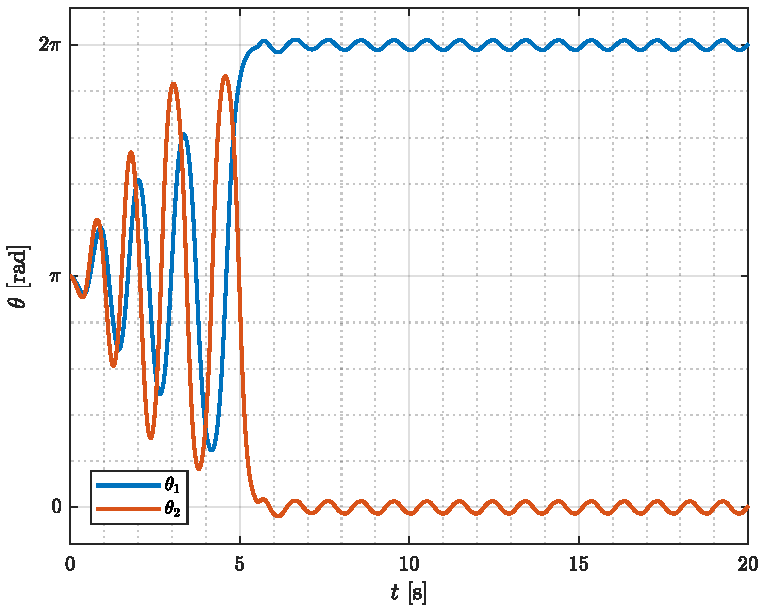
\includegraphics[width=.46\textwidth]{figures/theta_twinSwingAndCatch}
  }
  \hspace{20pt}
  \captionbox 
  {
    a
    \label{fig:ani_twinSwingAndCatch}
  }
  {
    \hspace{-1cm}
    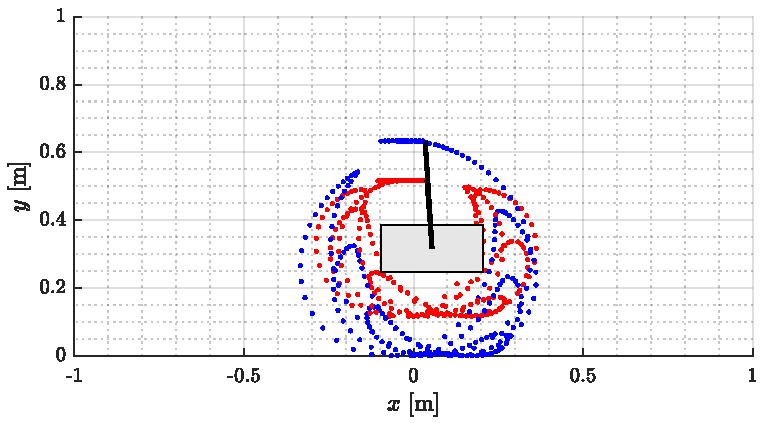
\includegraphics[width=.46\textwidth]{figures/ani_twinSwingAndCatch}
  }
\end{figure}
%
%
\begin{figure}[H]
  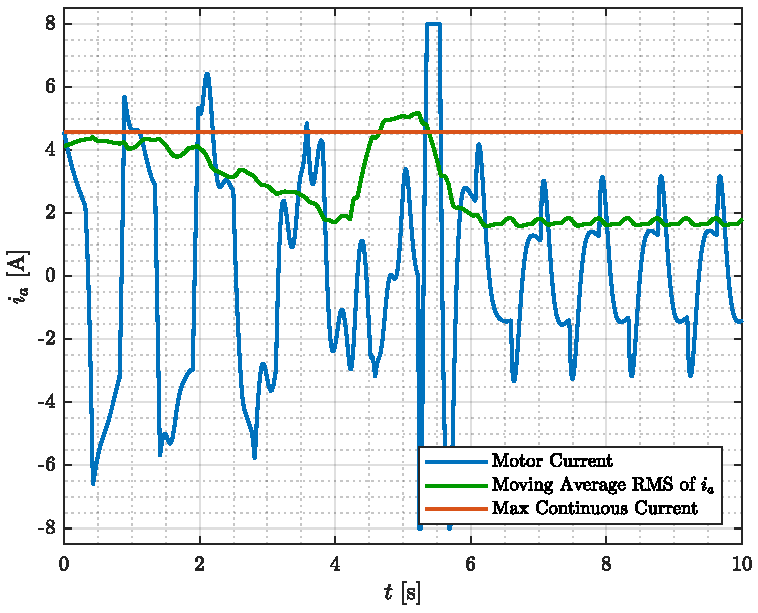
\includegraphics[width=.5\textwidth]{figures/ia_twinSwingAndCatch}
  \caption{a}
  \label{fig:ia_twinSwingAndCatch}
\end{figure}
%
\begin{figure}[H]
  \hspace{-10pt}
  \captionbox
  {
    a
    \label{fig:x_twinSwingAndCatch}
  }
  {
    \hspace{-1cm}
    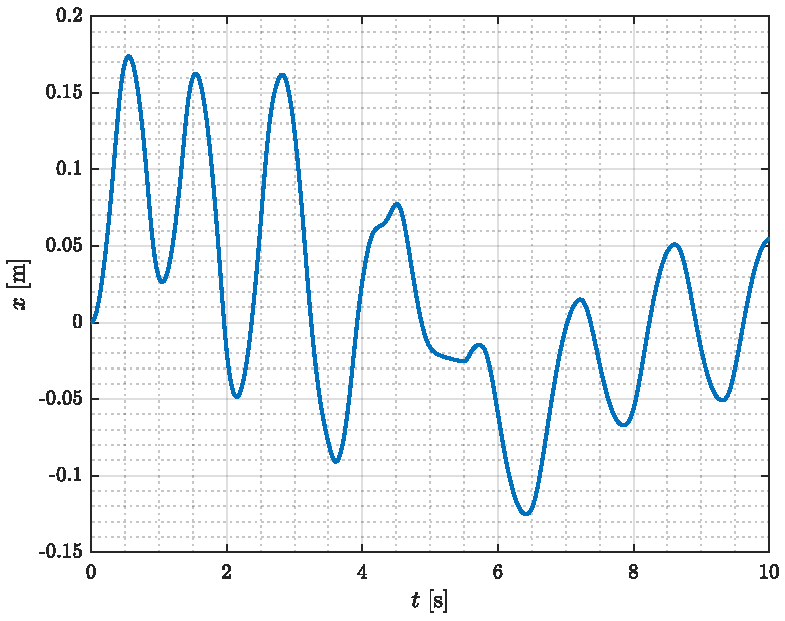
\includegraphics[width=.4\textwidth]{figures/x_twinSwingAndCatch}
  }
  \hspace{20pt}
  \captionbox 
  {
    a
    \label{fig:xDot_twinSwingAndCatch}
  }
  {
    \hspace{-1cm}
    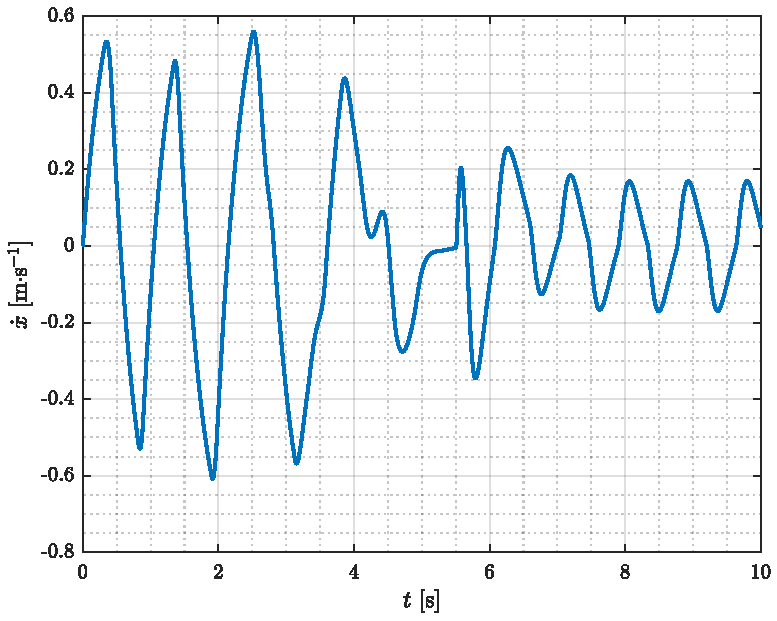
\includegraphics[width=.4\textwidth]{figures/xDot_twinSwingAndCatch}
  }  
\end{figure}
%
%
%\begin{figure}[H]
%  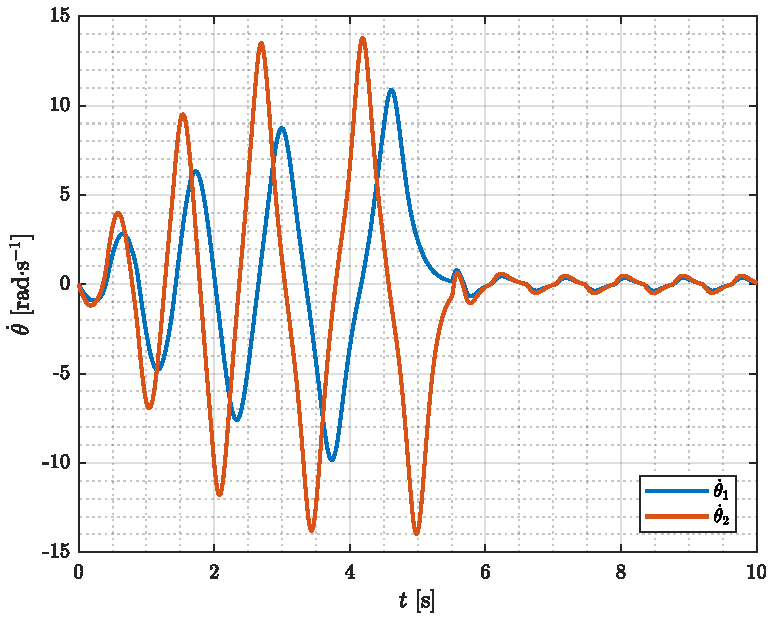
\includegraphics[width=.6\textwidth]{figures/thetaDot_twinSwingAndCatch}
%  \caption{thetaDotTwinSwingAndCatch}
%  \label{fig:thetaDot_twinSwingAndCatch}
%\end{figure}
%\begin{figure}[H]
%  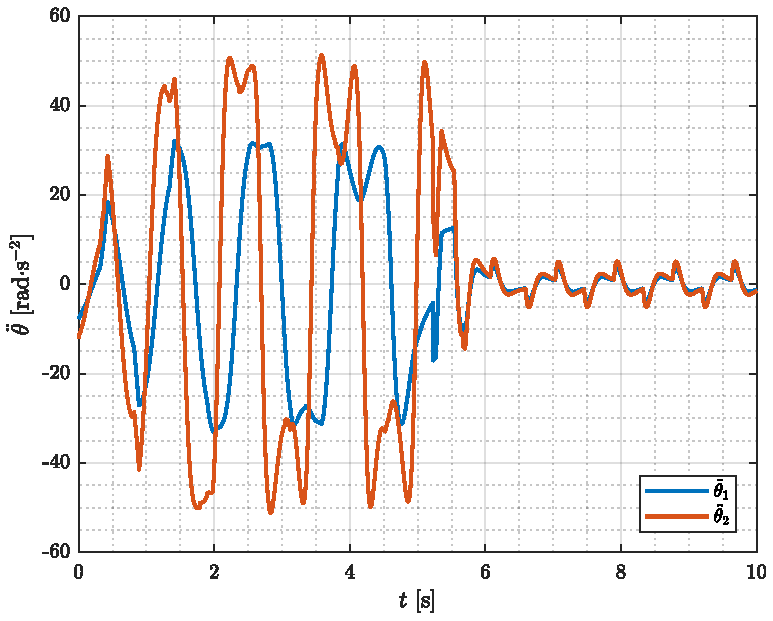
\includegraphics[width=.6\textwidth]{figures/thetaDotDot_twinSwingAndCatch}
%  \caption{thetaDotDotTwinSwingAndCatch}2.
%  \label{fig:thetaDotDot_twinSwingAndCatch}
%\end{figure}
%\begin{figure}[H]
%  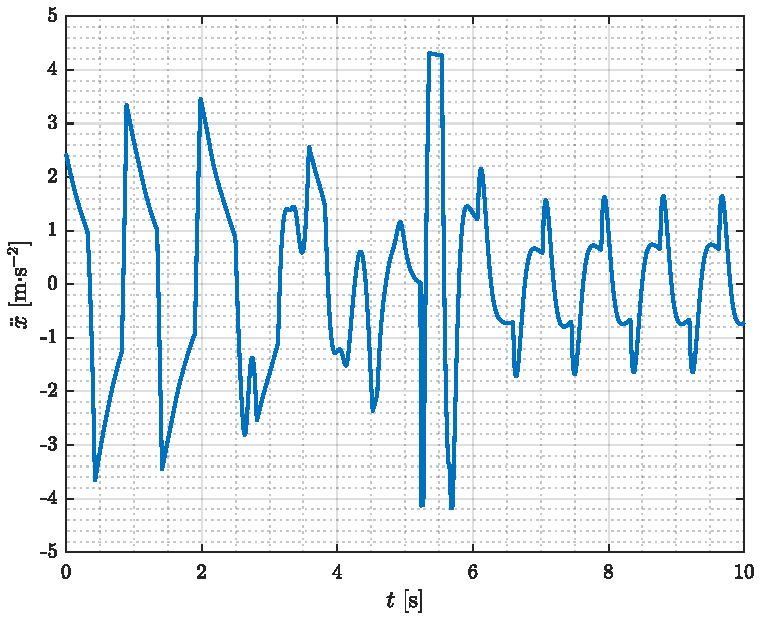
\includegraphics[width=.6\textwidth]{figures/xDotDot_twinSwingAndCatch}
%  \caption{xDotDotTwinSwingAndCatch}
%  \label{fig:xDotDot_twinSwingAndCatch}
%\end{figure}